\section{QT Demodulation}

\begin{figure}
	\centering
	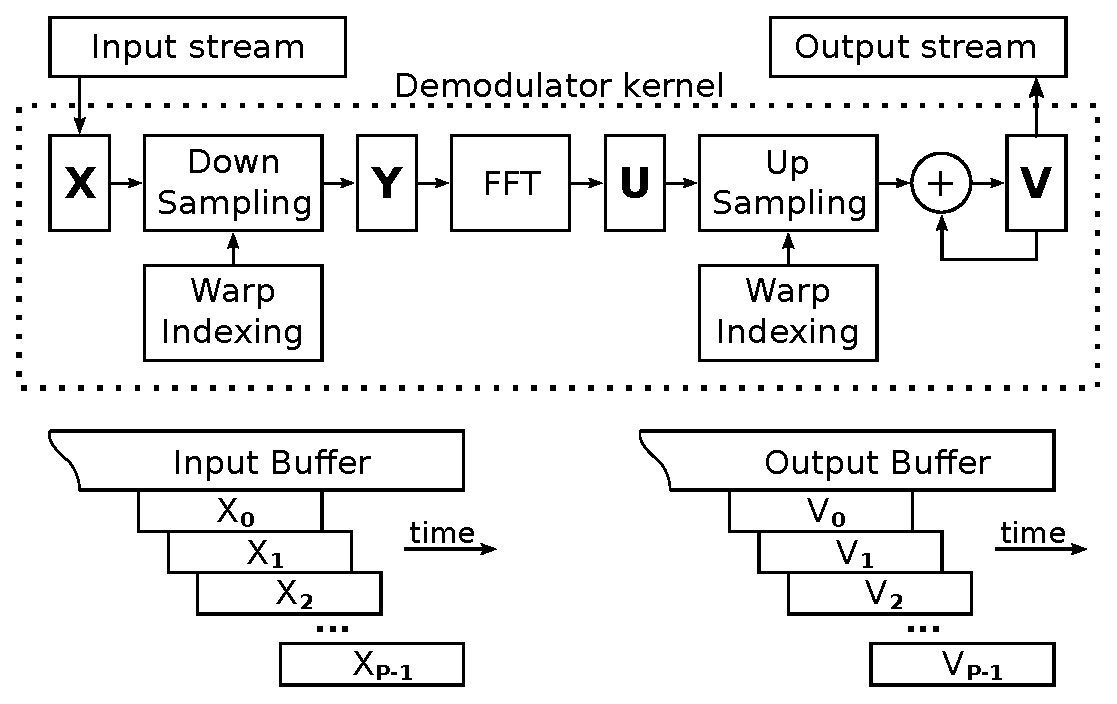
\includegraphics[width=0.95\linewidth]{../source/demod_e}
	\caption[Quantum to Relative Time Demodulation]{Demodulation data flow}
	\label{fig:demod}
\end{figure}

\begin{table}
	\label{tab:memory}
	\caption{Memory regions X, Y, U, and V in Fig.~\ref{fig:demod}
	are working buffers. For a 1k RFFT computed in place, the total is 11kB:}
	\centering
	\begin{tabular}{lccr}
		\hline\hline
		Buffer & Size & Bytes & Usage \\ [0.5ex]
		\hline
		X & 2048 x 16 & 4k & Input buffer\\
		Y/U & 1024 x 24 & 3k & FFT working buffer\\
		V & 512 x 64 & 4k & Output buffer\\
		\hline
	\end{tabular}
\end{table}

Multiple demodulator instances can be placed in an FPGA or ASIC to demodulate a
large number of $\omega$ values in parallel. This would be used in spectral
analysis, for finding signals; and deep data mining, for analyzing weak signals.
Due to the low I/O bandwidth, the algorithm lends itself to parallelism without
the complexity of high-speed signaling or memory management.
A low-cost ASIC would be feasible for consumer applications.

The mathematics of signal conversion, besides FFT, is College Algebra.
The algorithm can be coded by a typical programmer or engineer with some help
from the following derivations.

%%%%%%%%%%%%%%%%%%%%%%%%%%%%%%%%%%%%%%%%%%%%%%%%%%%%%%%%%%%%%%%%%%%%%%%%%%%%%%%%
\subsection{Downsampling}

The downsampling process of Fig.~\ref{fig:demod} translates the sample pitch of
X to the sample pitch of Y using an exponential sweep.
In the industry, this is known as exponential time-warping.

An exponential chirp sweeps from $f_0$ to $f_1$ in a time T.
M points of X get mapped onto N points of Y, where $M > N$.
Let R be a scaled version of $\omega$ for use in the exponential warp and
$\alpha$ the X input sample rate in samples per second.
Given a particular R and N, M and $\omega$ may be calculated.
Let $\epsilon = (f_1/f_0)^{1/T}$. The frequency with respect to time is:
\begin{equation}  \label{eq:fvsf0}
f = f_0 \cdot e^{\epsilon t}
\end{equation}

\subsubsection{Math}

The period of the incoming chirp changes exponentially with index n of $X[n]$.
Let $y = e^{|R|/N}$ be the pitch that accumulates along X.
It has units of ``e's per sample''.
As a scale factor, let $\omega = \frac{\alpha R}{N}$,
in units of ``e's per second'' e/s.
M is the number of input samples warping onto N points.
\begin{equation}  \label{eq:M_N}
%M = \sum_{n=0}^{N-1} y^n = \frac{y\cdot(y^{N-1} - 1)}{(y - 1)} + 1
M = N \cdot\frac{-y \cdot ln\left( N(1-y) + 1 \right)}{|R|}
\end{equation}

\begin{table}
	\label{tab:MNR}
	\caption{High values of M/N are undesirable because of excess processing
	time and memory usage.
    The point of diminishing returns for M/N is between 2 and 4.
    }
	\centering
	\begin{tabular}{lcr}
		\hline\hline
		$M/N$ & $Max |R|$ & $y_{max}:y_{min}$ \\ [0.5ex]
		\hline
		2 & 1.256 & 3.51:1\\
		4 & 2.337 & 10.35:1\\
		8 & 4.229 & 68.66:1\\
		\hline
	\end{tabular}
\end{table}

An upper limit of 2 for M/N is reasonable from both a mathematical and
hardware standpoint. For example, if M is constrained to 2N, N=1024, and
$\alpha$ = 10000 samples/second, then $|\omega|$ ranges between 0 and 12.26 e/s.
When fixed-sized memories are used, smaller N allows for larger M/N, larger R,
and higher $\omega$ per input sample rate.

Re-sampling is done on N points (of Y) at a time where the respective indices of
X and Y are $\delta$ and i.
The time span is from 0 to i/N where i sweeps from 0 to N-1 and N is the number
of samples.
Let $\lambda$ be the sample pitch of X.
It will increase or decrease exponentially and should have a minimum value of
1.0, but allowed a minimum value of less than one to allow for rounding error.

This causes a chirp of matching R to be re-sampled to the upper frequency
(either $f_0$ or $f_1$ depending on the sign of R).
Given output index i, input sample index $\delta(i)$ is the accumulated sum of
$\lambda(i)$ when $\lambda$ starts at 1.0 and increases exponentially
or starts at $e^{-R}$ and decreases exponentially.
The exponential sweep can be implemented with a multiplier.
For each step:
\begin{equation}  \label{eq:lambda}
\lambda = \lambda + (\lambda\cdot\Lambda)
\end{equation}

The initial value of $\lambda$ is $e^{-R}$ when $R<0$; otherwise, it's 1.
The ``repeated multiply'' approach to exponential sweep is nearly base $e$,
but it needs a small correction factor to hit $e$.
Setting $e^R = (1 + \Lambda)^N$,
\begin{equation}  \label{eq:lambdaApprox}
\Lambda = e^{R/N} - 1
\end{equation}

As a sanity check, a downward-chirping sine wave was generated using a phase
angle proportional to $e^{n\cdot R/N} - 1$ with index $n$ starting from 0.
$\Lambda$ was set to $e^{R/N} - 1$.
A 512-point FFT (with Hann window) was performed on the de-chirped wave to
produce the expected narrow peak.

Verification of an exponential sweep built around a 27x26 multiplier used R=1.6
and N=8192. For upward sweep starting at 1.0, $\Lambda$ was $26846167/2^{37}$
according to Eq. \ref{eq:lambdaApprox}.
The accumulated $\Lambda$ was tracked and compared to the expected value from
Eq. \ref{eq:M_N}. The accumulated error after 8192 steps was less than 0.001
of an X sample pitch, so more than an order of magnitude better than necessary.
Rounding was the source of error.
Adding 1 to the LSB of $\Lambda$ lowered it to below 0.00025.
Downward sweep starting at $e^{1.6}$ had much less error.
$\Lambda$ was $-26840924/2^{37}$ and error peaked at 50 PPM.

\subsubsection{Interpolation}

The i index is stepped from 0 to N-1, where N is a power of 2 (although it
doesn't have to be) for the convenience of the FFT. $\delta(i)$ sweeps
non-linearly from 0 to M. For each X, its index $\delta$ is the running sum
of $\lambda$. For each Y point, the downsampler averages one or more X points.

There are two ways to do handle downsampling: Linear interpolation of the output
of a variable frequency low pass filter, and summation of $\lambda$
input samples.

The most common downsampling method is the low pass filter whose output is
sampled less often than its input rate.
This method attenuates alias frequencies before they make it to the output.
Anti-aliasing is good to have, but not essential in this case.
Since the alias of an exponential chirp is no longer a pure exponential
chirp (it's a linear combination of factors), it will show up in the data stream
as wideband noise rather than narrowband interference.
A low pass filter might not be needed.
The computing resourced for the filter aren't cheap.
However, a filter would improve SNR.
Such a filter must have a linear phase response.
A neat trick to use with IIR filters is forward-backward filtering,
which zeros the phase shift.
The endpoints of the filtered X are allowed some slop,
as the Hann window will lop them off anyway.

The non-filter approach is to simply sum $\lambda$ input samples of X.
Some fractional arithmetic is required to handle partial contributions.
Fig.~\ref{fig:xint} illustrates a simple interpolation that adds two fractional
endpoints to 0 or more midpoints for downsampling.
$k$ is the integer part of $\delta$.

\begin{figure}
	\centering
	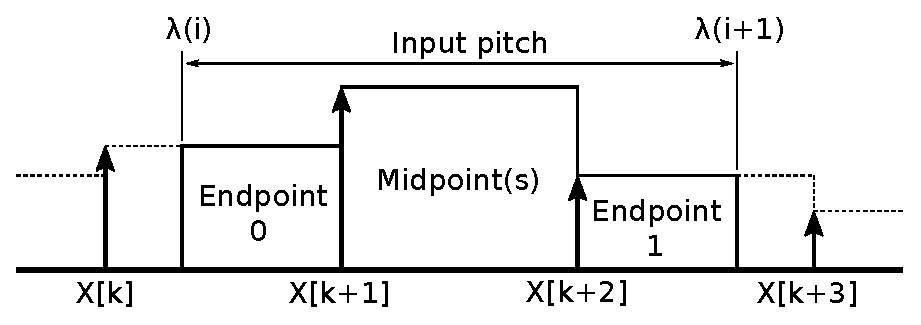
\includegraphics[width=0.95\linewidth]{../source/xint_e}
	\caption[X interpolation]{Sum of $X_\delta$ for downsampling}
	\label{fig:xint}
\end{figure}

In either case, the output of the downsampler could be scaled by
$s=\sqrt{1/\lambda}$ to flatten the noise floor.
The Central Limit Theorem reduces noise
by the square root of the number of samples in a sum.
On the other hand, one might expect energy conservation to cause the
amplitude of the incoming signal to fall off with time spreading.
So, the scaling should be optional.
Another instance of exponential sweep, with $\Lambda_s = -\Lambda/2$
and $s_0 = e^{R/2N}$,
can produce this scale factor rather easily.

\begin{figure}
	\centering
	\includegraphics[width=0.95\linewidth]{../source/xbuf_e}
	\caption[X buffer usage]{X buffer usage}
	\label{fig:xbuf}
\end{figure}

Oversampling would normally use a sliding window on a circular buffer sized as
a power of two to allow pointer wrapping by bitwise-and.
Fig.~\ref{fig:xbuf} shows the memory layout of $X$.
After a block of processing, $\alpha\Delta$ input samples are concatenated to
$X$ and the index of $X_0$ is offset by $\alpha\Delta$,
where $\Delta$ is the time interval of the blocks.

%%%%%%%%%%%%%%%%%%%%%%%%%%%%%%%%%%%%%%%%%%%%%%%%%%%%%%%%%%%%%%%%%%%%%%%%%%%%%%%
\subsection{FFT}

After X is time warped into Y, Y is processed by a Fast Fourier Transform and
converted to data set U containing N/2 frequency bins. Y and U may share the
same physical memory if the FFT is performed in place.

Polar format is preferred for the output of the FFT,
for the benefit of the upsampler.
A Hann window $w(n)$ is applied to Y before performing the FFT.
\begin{equation}
w(n) = \frac{1}{2}\left(1 - cos\left( \frac{2\pi n}{N-1} \right)\right)
\end{equation}


The reference VHDL implementation uses a pipelined CORDIC to perform the FFT.
It also applies a Hann window to Y, converts to polar output, and is shared with
the correlator to perform polar to rectangular conversions.

A DIT FFT is the usual choice for RFFT since bit reversal is easier at the input.
With an RFFT, you get twice the outputs given real-only input.
Adjacent input samples are grouped as pairs, with even samples as real and odd
samples as imaginary components of the complex input points.
After a CFFT is performed, a separation step doubles the output size.
Our experience is that the precision of the separation step degrades with small N
(maybe we did it wrong), so a simple CFFT (with zeroed imaginary part)
may be preferable in cases of small N.

An FFT can be converted to IFFT somewhat trivially, so the same hardware can
support either modulation or demodulation.

%%%%%%%%%%%%%%%%%%%%%%%%%%%%%%%%%%%%%%%%%%%%%%%%%%%%%%%%%%%%%%%%%%%%%%%%%%%%%%%%
\subsection{Upsampling}

U is upsampled to form time-domain signal V.
Let $\epsilon$ and j be the respective indices of U and V.
For every index $\epsilon$ of U, the corresponding frequency can be normalized
to Fs/2. 

Let $H_X$ be the integer number of new X samples per conversion.

Let $H_V$ be the integer number of output samples per conversion.
Since $H_V < H_X$ and the minimum $H_V$ is 1, $H_V$ is a main consideration in
choosing $H_X$ and is the limiting factor for the lowest practical R.

Substituting the FFT frequency range into Eq. \ref{eq:fvsf0}, 
\begin{equation}  \label{eq:hv}
H_V = \frac{N}{2} \left( e^{|R| \cdot H_X / N} - 1 \right)
\end{equation}
Since the exponent is very small and $H_V$ is rounded to integer anyway,
\begin{equation}
H_V \approx H_X \cdot \frac{|R|}{2}
\end{equation}

For small values of R, such as $|R| < 0.2$,
you can set $H_V = 1$ to get the minimum $H_X$.
\begin{equation}
H_X \geq \frac{2}{|R|}
\end{equation}

It's much easier to work in terms of exponents than logs,
so the preferred re-mapping (another exponential time-warping operation)
extracts $U[\epsilon]$ from a linear progression of $V[j]$.
Warp indexing uses the relation:
\begin{equation}
\epsilon = \frac{N}{2} \cdot e^{\omega(t - \tau)}
\end{equation}

Time t (scaled to match the output stream's sample rate) sweeps from $\tau$
in the opposite direction of R's sign,
causing the exponent to start at 1 and decay downward.

Up-sampling $U[\epsilon]$ to $V[j]$ can't use the popular interpolation scheme
(zero stuffing) because the interpolation factor must be irrational. Instead,
partial contributions to $V[j]$ are extracted from one or two U points by
interpolation.

$j$ sweeps downward from $N/2-1$. Index $\epsilon(j)$ is independent of R.
The approximation factor k should be about 2. 
It's tweaked to make both $H_X$ and $H_V$ integers.

\begin{equation}  \label{eq:eps_j}
\epsilon(j) = \frac{N}{2} \cdot e^{-kj/N}
\end{equation}

As a sanity check of Eq. \ref{eq:eps_j}, $\epsilon(j)$ starts at (N/2-1) which
points to the highest frequency element of the FFT result.
It decays toward 0 but will never get there.
The number of elements in W memory is slightly less than N/2 to allow some I/O
headroom. Due to the limited size of W memory,
the lowest frequency is about $(1/e)$ of the highest frequency,
leaving the lower $\approx37$\% of the spectrum unused.

The exact value of $k$ is:
\begin{equation} 
k = \frac{N}{H_V} \left(e^{|R| \cdot H_X/N} - 1\right)
\end{equation}

Once $H_V$ is estimated to the nearest integer, $H_X$ and $k$ can be
re-calculated from Eq. \ref{eq:hv} to give a $k$ nearest to 2.0:
\begin{equation}  \label{eq:hx}
H_X = \frac{N}{|R|} ln \left( \frac{k \cdot H_X}{N} - 1 \right)
\end{equation}

The exponential decay of $\epsilon$, where $\epsilon_0 = \frac{N}{2}-1$, can be
handled by repeated multiplication.
The exponential sweep needs a small correction factor to have a base of exactly
$e$.
Setting $e^{-k} = (1 + \zeta)^N$,
\begin{equation}
\zeta = e^{k/N} - 1
\end{equation}

Since $\epsilon$ is always positive, the upchirp case of $R>0$ needs to have its
j index mirrored by using V[v-j], where v is the maximum j such as (15/32)N.

\begin{figure}
	\centering
	\includegraphics[width=0.95\linewidth]{../source/uint_e}
	\caption[U interpolation]{Extraction of $U_\epsilon$}
	\label{fig:uint}
\end{figure}

Fig.~\ref{fig:uint} shows upsampling of U to V. It uses linear interpolation to
construct a curve to extract from.
In this case, the upsampler input pitch is less than 1.0 samples.
The height of $U_\epsilon$ is interpolated and multiplied by the pitch to get
the area under the curve, to be added to V[j].
The operation is similar to the "$\lambda < 1$" case of downsampling,
so the same hardware can support downsampling and upsampling.

%%%%%%%%%%%%%%%%%%%%%%%%%%%%%%%%%%%%%%%%%%%%%%%%%%%%%%%%%%%%%%%%%%%%%%%%%%%%%%%%
\subsection{Correlation}

Warped U is added to output buffer V by the summation,
staggered in time (by P samples) for each processing block.
When the downsampler's R value matches the chirp rate of an incoming chirp,
multiple peaks in the warped FFT output correlate in the output stream to
produce a corresponding output pulse in the V stream.
A more complex signal such as overlapping and/or modulated chirps will produce
pulse trains and/or modulation envelopes in the V stream.

\begin{figure}
	\centering
	\includegraphics[width=0.99\linewidth]{../source/wbuf_e}
	\caption[W correlation]{Correlation of V}
	\label{fig:wbuf}
\end{figure}

Fig.~\ref{fig:wbuf} shows the output correlator, another view of buffer V.
The output stream flows from left to right,
being initialized to 0 outside the accumulation region.
After $U_\epsilon$ is added to V, the $V_0$ index moves $\beta\Delta$ points
to the left, leaving $\beta\Delta$ newly minted output points.

Elements of V may be real (magnitudes only) or complex.
Complex is used when high selectivity is required:
Multiple rotating vectors will sum to zero, while vectors pointing in the same
direction (chirps matching R) will correlate.
Correlation through vector averaging allows the use of a much smaller FFT than
scalar-only averaging.
The rate of phase rotation is proportional to the FFT result frequency,
so selectivity is higher at the upper end.
Since the low end of the FFT result isn't used,
lower selectivity there isn't a problem.

Due to the requirement that phase rotation be stationary across many FFT results
for signal detection, the exponential sweeps used in downsampling and upsampling
should use sufficient precision for correct tracking.

The correlator should be able to work with either vectors or real magnitudes
(no phase data).
This would be used in signal search, where low selectivity is desired.
The data in V, where the accumulations occur, is in rectangular format.
The data coming from the upsampler is in polar format.
The correlation process may use a CORDIC to perform polar-to-rectangular
conversion.
